\documentclass[]{standalone}
\usepackage{mathptmx}
%\renewcommand{\familydefault}{\rmdefault}
\usepackage[T1]{fontenc}
\usepackage[latin9]{inputenc}
\usepackage{siunitx}
\usepackage{array}
\usepackage{amsmath}
\usepackage{ifthen}
\usepackage{pgfplots}
\pgfplotsset{compat=1.14}
\usepackage{titling, graphicx}
\usepackage{tikz}
\usepackage{upgreek}
\usepackage{amsmath,amsthm}
\usepackage{strtikz}
\usetikzlibrary{shapes,arrows.meta,intersections,graphs,graphs.standard,math,fit}
\usetikzlibrary{calc,intersections,through,backgrounds}
\usetikzlibrary{decorations.pathmorphing, decorations.markings,decorations.pathreplacing}


\begin{document}
\begin{tikzpicture}

\commonisolation[%
startX = 0cm,
startY = 0cm,
support width = 0.5cm,
support body = 11.5cm,
support height = 0.2cm,
support line thickness = 1.0pt,
number of isolators = 8,
isolator width = 0.5cm,
isolator thickness = 0.2cm,
isolator line thickness = 1pt,
isolator drift=0.5cm,
isolator number to show drift=1,
show isolation drift=1,
foundation thickness = 0.3cm,
foundation side width = 1.3cm,
mass text for slab = $m_\text{b}$,
text location for mass=left,
show mass text=1,
arrow tip length=3pt,
arrow tip width=2pt,
isolation drift text=$x_\text{b}$,]

 
\framestructure[%
number of storys=3,
number of bays=2,
story height=1cm,
bay width=1.5cm,
startX=0cm,
startY=0cm,
frame line thickness = 1.5pt,
show supports = 0,
show mass = 0,
show dof=0,
show axes=0,
show piles=0,]

\framestructure[%
number of storys=4,
number of bays=2,
story height=1cm,
bay width=1.5cm,
startX=3.5cm,
startY=0cm,
frame line thickness = 1.5pt,
show supports = 0,
show mass = 0,
show dof=0,
show axes=0,
show piles=0,]

\framestructure[%
number of storys=2,
number of bays=3,
story height=1cm,
bay width=1.5cm,
startX=7.0cm,
startY=0cm,
frame line thickness = 1.5pt,
show supports = 0,
show mass = 0,
show dof=0,
show axes=0,
show piles=0,]

\end{tikzpicture}
\end{document}